\documentclass{article}
\usepackage[utf8]{inputenc}
\usepackage{amsmath}
\usepackage{cite}
\usepackage[letterpaper,top=1cm,bottom=2cm,left=1.5cm,right=1.5cm]{geometry}
\usepackage{wrapfig}
\usepackage{graphicx}

\begin{document}

\title{Campo Eléctrico de un Dipolo}
\author{Ariel Alejandro Calderón}
\date{15 de Octubre del 2024}
\maketitle

\section*{Definición de un Dipolo Eléctrico}

\begin{wrapfigure}{r}{0.4\textwidth}
    \centering
    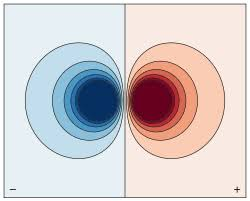
\includegraphics[width=0.33\textwidth]{./public/dipolo.png}
    \caption{Carga por fricción.}
\end{wrapfigure}

Un \textbf{dipolo eléctrico} es un sistema formado por dos cargas puntuales de igual magnitud pero signo opuesto, separadas por una distancia \( d \). Las cargas son \( +q \) y \( -q \), y el \textit{momento dipolar} \( \mathbf{p} \) está dado por:

\[
\mathbf{p} = q \mathbf{d}
\]

donde \( \mathbf{d} \) es el vector que va desde la carga negativa hasta la carga positiva, y su magnitud es \( d \).

\section*{Potencial Eléctrico de un Dipolo}

El potencial eléctrico en un punto \( (x, y) \) debido a un dipolo se aproxima como:

\[
V(x, y) = \frac{1}{4\pi\epsilon_0} \frac{\mathbf{p} \cdot \hat{r}}{r^2}
\]

donde:
\begin{itemize}
    \item \( \mathbf{p} \) es el momento dipolar.
    \item \( \hat{r} \) es el vector unitario que apunta hacia el punto \( (x, y) \).
    \item \( r = \sqrt{x^2 + y^2} \) es la distancia desde el origen (ubicación del dipolo) hasta el punto \( (x, y) \).
\end{itemize}

\section*{Campo Eléctrico de un Dipolo}

El campo eléctrico \( \mathbf{E}(x, y) \) está relacionado con el potencial \( V(x, y) \) por la siguiente expresión:

\[
\mathbf{E}(x, y) = -\nabla V(x, y)
\]

Para un dipolo ubicado en el origen, las componentes del campo eléctrico \( E_x \) y \( E_y \) en un punto \( P(x, y) \) se pueden escribir como:

\[
E_x = \frac{1}{4\pi\epsilon_0} \left( \frac{3p x y}{r^5} \right)
\]

\[
E_y = \frac{1}{4\pi\epsilon_0} \left( \frac{p(2y^2 - x^2)}{r^5} \right)
\]


Donde:
\begin{itemize}
    \item \( p = qd \) es el momento dipolar.
    \item \( r = \sqrt{x^2 + y^2} \) es la distancia al punto \( P(x, y) \).
\end{itemize}

\section*{Bibliografía}
\begin{itemize}
    \item Tipler, P. A., \& Mosca, G. (2008). \textit{Física para la ciencia y la tecnología}. Volumen 2. Reverté.
    \item Serway, R. A., \& Jewett, J. W. (2014). \textit{Física para ciencias e ingeniería}. Cengage Learning.
    \item Young, H. D., \& Freedman, R. A. (2012). \textit{Sears y Zemansky: Física universitaria}. Pearson Educación.
\end{itemize}


\end{document}
